\documentclass{scrartcl}
        \usepackage{xcolor, tikz}
        \usepackage{pgfplots}
        \pgfplotsset{compat=newest}
        \pagestyle{empty}
        \definecolor{pdg2112}{RGB}{228,26,28}
\definecolor{pdg1000060130}{RGB}{153,153,153}
\definecolor{pdg2212}{RGB}{55,126,184}
\definecolor{pdg1000010020}{RGB}{153,153,153}
\definecolor{pdg1000020040}{RGB}{166,86,40}
\definecolor{pdg11}{RGB}{152,78,163}
\definecolor{pdg1000060110}{RGB}{153,153,153}
\definecolor{pdg1000030070}{RGB}{153,153,153}
\definecolor{pdg22}{RGB}{77,175,74}
\definecolor{pdg1000020060}{RGB}{153,153,153}
\begin{document}
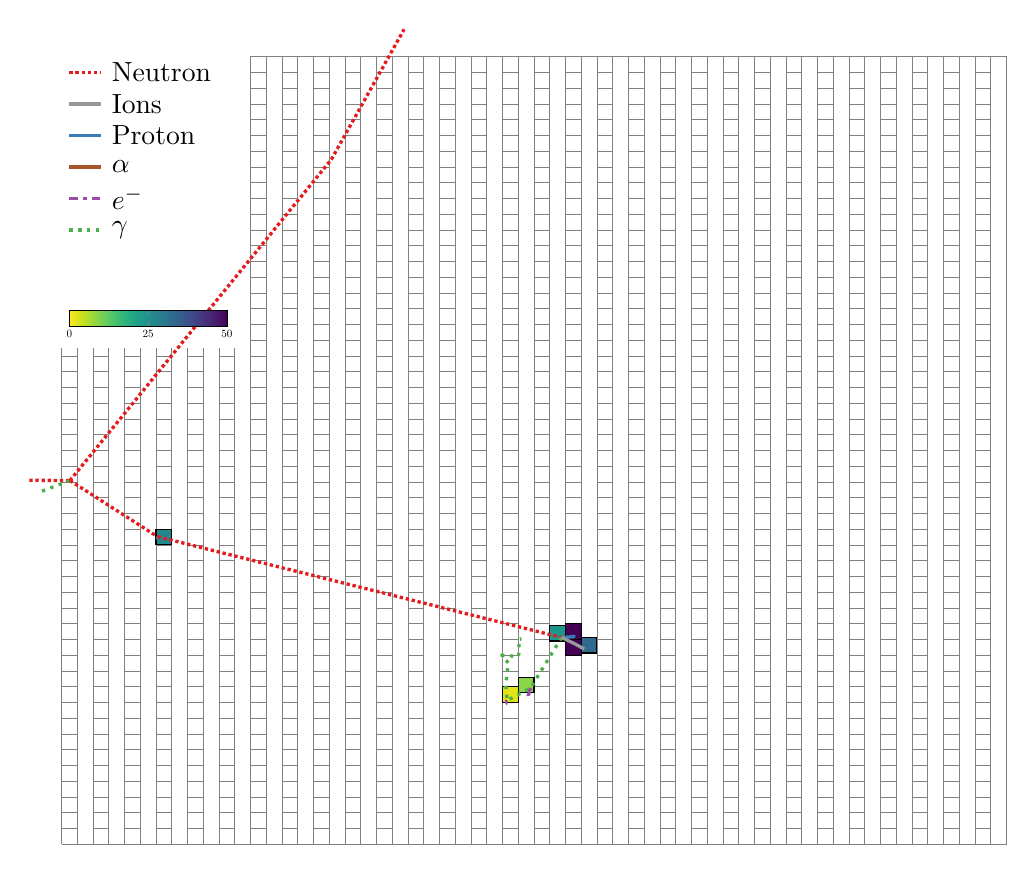
\begin{tikzpicture}[scale=0.4] %\columnwidth/252.0pt]
\draw[step=0.5,very thin,gray] (-0.001000,-12.499) grid (0.500000,3.25);
\draw[step=0.5,very thin,gray] (0.999000,-12.499) grid (1.500000,3.25);
\draw[step=0.5,very thin,gray] (1.999000,-12.499) grid (2.500000,3.25);
\draw[step=0.5,very thin,gray] (2.999000,-12.499) grid (3.500000,3.25);
\draw[step=0.5,very thin,gray] (3.999000,-12.499) grid (4.500000,3.25);
\draw[step=0.5,very thin,gray] (4.999000,-12.499) grid (5.500000,3.25);
\draw[step=0.5,very thin,gray] (5.999000,-12.499) grid (6.500000,12.499);
\draw[step=0.5,very thin,gray] (6.999000,-12.499) grid (7.500000,12.499);
\draw[step=0.5,very thin,gray] (7.999000,-12.499) grid (8.500000,12.499);
\draw[step=0.5,very thin,gray] (8.999000,-12.499) grid (9.500000,12.499);
\draw[step=0.5,very thin,gray] (9.999000,-12.499) grid (10.500000,12.499);
\draw[step=0.5,very thin,gray] (10.999000,-12.499) grid (11.500000,12.499);
\draw[step=0.5,very thin,gray] (11.999000,-12.499) grid (12.500000,12.499);
\draw[step=0.5,very thin,gray] (12.999000,-12.499) grid (13.500000,12.499);
\draw[step=0.5,very thin,gray] (13.999000,-12.499) grid (14.500000,12.499);
\draw[step=0.5,very thin,gray] (14.999000,-12.499) grid (15.500000,12.499);
\draw[step=0.5,very thin,gray] (15.999000,-12.499) grid (16.500000,12.499);
\draw[step=0.5,very thin,gray] (16.999000,-12.499) grid (17.500000,12.499);
\draw[step=0.5,very thin,gray] (17.999000,-12.499) grid (18.500000,12.499);
\draw[step=0.5,very thin,gray] (18.999000,-12.499) grid (19.500000,12.499);
\draw[step=0.5,very thin,gray] (19.999000,-12.499) grid (20.500000,12.499);
\draw[step=0.5,very thin,gray] (20.999000,-12.499) grid (21.500000,12.499);
\draw[step=0.5,very thin,gray] (21.999000,-12.499) grid (22.500000,12.499);
\draw[step=0.5,very thin,gray] (22.999000,-12.499) grid (23.500000,12.499);
\draw[step=0.5,very thin,gray] (23.999000,-12.499) grid (24.500000,12.499);
\draw[step=0.5,very thin,gray] (24.999000,-12.499) grid (25.500000,12.499);
\draw[step=0.5,very thin,gray] (25.999000,-12.499) grid (26.500000,12.499);
\draw[step=0.5,very thin,gray] (26.999000,-12.499) grid (27.500000,12.499);
\draw[step=0.5,very thin,gray] (27.999000,-12.499) grid (28.500000,12.499);
\draw[step=0.5,very thin,gray] (28.999000,-12.499) grid (29.500000,12.499);
\draw[very thin,gray] (0,-12.5) -- (30,-12.5) -- (30,12.5) -- (6,12.5);
\definecolor{tempcolor}{rgb}{0.140536,0.530132,0.555659}\draw[fill=tempcolor,fill opacity=1] (3.000000,-3.000000) rectangle (3.500000,-2.500000);
\definecolor{tempcolor}{rgb}{0.886271,0.892374,0.095374}\draw[fill=tempcolor,fill opacity=1] (14.000000,-8.000000) rectangle (14.500000,-7.500000);
\definecolor{tempcolor}{rgb}{0.545524,0.838039,0.275626}\draw[fill=tempcolor,fill opacity=1] (14.500000,-7.696365) rectangle (15.000000,-7.196365);
\definecolor{tempcolor}{rgb}{0.121831,0.589055,0.545623}\draw[fill=tempcolor,fill opacity=1] (15.500000,-6.050882) rectangle (16.000000,-5.550882);
\definecolor{tempcolor}{rgb}{0.267004,0.004874,0.329415}\draw[fill=tempcolor,fill opacity=1] (16.000000,-6.500000) rectangle (16.500000,-6.000000);
\definecolor{tempcolor}{rgb}{0.267004,0.004874,0.329415}\draw[fill=tempcolor,fill opacity=1] (16.000000,-6.000000) rectangle (16.500000,-5.500000);
\definecolor{tempcolor}{rgb}{0.187231,0.414746,0.556547}\draw[fill=tempcolor,fill opacity=1] (16.500000,-6.430077) rectangle (17.000000,-5.930077);
\draw[color=pdg2112, very thick, densely dotted] (-1.0215048412911074, -0.9468965310859927) -- (-0.02164916908500345, -0.9532515413617377) -- (0.0029999999999972713, -0.9534082096961566) -- (0.26689914806449905, -0.9550855335783224);
\draw[color=pdg1000060110, very thick, solid] (0.26689914806449905, -0.9550855335783224);
\draw[color=pdg22, very thick, dotted] (0.26689914806449905, -0.9550855335783224) -- (0.17497724913368984, -0.99) -- (0.1565478312315463, -0.9969999999999999) -- (0.14075118731541353, -1.0030000000000001) -- (0.12758731738531423, -1.0080000000000002) -- (0.010000000000013642, -1.0526628985281745) -- (-0.7594632295789324, -1.3449262047080166);
\draw[color=pdg2112, very thick, densely dotted] (0.26689914806449905, -0.9550855335783224) -- (0.3214046950042757, -0.99) -- (0.3416992085064976, -1.0030000000000001) -- (0.48999999999998634, -1.0979966250339366) -- (0.9899999999999863, -1.4182802326844888) -- (1.1019629066276593, -1.4899999999999998) -- (1.1222574201298812, -1.5030000000000001) -- (1.4899999999999636, -1.7385638403350374) -- (1.8583398039984786, -1.974510242866926) -- (1.8844146814765055, -1.9912129545223394) -- (1.949601875171561, -2.03296973366087) -- (2.0029999999999974, -2.0671748217845165) -- (2.4899999999999864, -2.379131055636142) -- (2.9899999999999864, -2.699414663286694) -- (3.049993300067649, -2.737844404447757);
\draw[color=pdg1000030070, very thick, solid] (3.049993300067649, -2.737844404447757);
\draw[color=pdg1000020040, very thick, solid] (3.049993300067649, -2.737844404447757);
\draw[color=pdg2212, very thick, solid] (3.049993300067649, -2.737844404447757) -- (3.046863737278818, -2.765064921279561) -- (3.0443080735846935, -2.7868892410226564) -- (3.0421323121741124, -2.8041616801606786) -- (3.0402267491030215, -2.8180051961229013) -- (3.0386545718649813, -2.8291296846804035);
\draw[color=pdg2112, very thick, densely dotted] (3.049993300067649, -2.737844404447757) -- (3.4899999999999864, -2.847606081319557) -- (3.9899999999999864, -2.97233336034585) -- (4.060821073754141, -2.9899999999999993) -- (4.088882296826773, -2.9969999999999994) -- (4.112934773746178, -3.0029999999999997) -- (4.132978504512357, -3.008) -- (4.489999999999986, -3.097060639372145) -- (4.989999999999986, -3.2217879183984373) -- (5.489999999999986, -3.34651519742473) -- (5.989999999999986, -3.471242476451022) -- (6.065194150371167, -3.4899999999999998) -- (6.093255373443799, -3.496999999999999) -- (6.117307850363204, -3.503) -- (6.137351581129383, -3.5080000000000005) -- (6.490000000000009, -3.595969755477315) -- (6.642540647021929, -3.634021715165224) -- (6.660393745626516, -3.6384752519875) -- (6.675696401573282, -3.6422925692637365) -- (6.688448614862272, -3.645473666993934) -- (6.989999999999986, -3.7206970345036092) -- (7.489999999999986, -3.845424313529901) -- (7.917761975920894, -3.952131488184949) -- (7.935615074525458, -3.9565850250072243) -- (7.950917730472247, -3.9604023422834613) -- (7.963669943761215, -3.9635834400136587) -- (7.989999999999986, -3.9701515925562028) -- (8.069567226988147, -3.9899999999999998) -- (8.097628450060778, -3.997) -- (8.121680926980185, -4.003) -- (8.141724657746362, -4.008000000000001) -- (8.489999999999986, -4.094878871582496) -- (8.989999999999986, -4.219606150608788) -- (9.489999999999986, -4.34433342963508) -- (9.989999999999986, -4.469060708661373) -- (10.07394030360515, -4.49) -- (10.102001526677782, -4.497) -- (10.126054003597186, -4.503) -- (10.146097734363366, -4.508000000000001) -- (10.490000000000009, -4.593787987687671) -- (10.514112601559168, -4.599802986053109) -- (10.990000000000009, -4.7185152667139665) -- (11.489999999999986, -4.843242545740253) -- (11.743425962617767, -4.906460807244124) -- (11.761279061222377, -4.9109143440664) -- (11.776581717169142, -4.914731661342637) -- (11.789333930458133, -4.917912759072834) -- (11.989999999999986, -4.967969824766549) -- (12.078313380222152, -4.99) -- (12.106374603294807, -4.997) -- (12.130427080214213, -5.003) -- (12.15047081098037, -5.008000000000001) -- (12.489999999999986, -5.092697103792841) -- (12.989999999999986, -5.217424382819134) -- (13.489999999999986, -5.342151661845426) -- (13.990000000000009, -5.466878940871718) -- (14.082686456839202, -5.49) -- (14.11074767991181, -5.497) -- (14.134800156831194, -5.503) -- (14.154843887597348, -5.508) -- (14.489999999999963, -5.591606219898023) -- (14.990000000000009, -5.7163334989243095) -- (15.490000000000009, -5.841060777950602) -- (15.569089949314707, -5.860790126303303) -- (15.586943047919272, -5.865243663125579) -- (15.602245703866084, -5.869060980401815) -- (15.614997917155051, -5.872242078132013) -- (15.877564691619273, -5.937740556815276);
\draw[color=pdg1000020060, very thick, solid] (15.877564691619273, -5.937740556815276);
\draw[color=pdg22, very thick, dotted] (15.877564691619273, -5.937740556815276) -- (15.798617904791286, -6.06640848593756) -- (15.78845135303818, -6.082977990700771) -- (15.510000000000014, -6.536799614052972) -- (15.502999999999997, -6.548208254480862) -- (15.497000000000025, -6.557987089133322) -- (15.491999999999985, -6.566136118010417) -- (15.231929819623383, -6.99) -- (15.010000000000014, -7.351702501757754) -- (15.002999999999997, -7.363111142185643) -- (14.997000000000025, -7.372889976838103) -- (14.991999999999985, -7.3810390057151976) -- (14.893360309379137, -7.5418025431736755) -- (14.510000000000014, -7.748690978849643) -- (14.150305779836344, -7.942807512853534) -- (14.110919101510012, -7.51) -- (14.104178801912507, -7.435933020284016) -- (14.157284750733675, -7.010000000000001) -- (14.189796755877978, -6.749239447669629) -- (14.010000000000014, -6.542033902194509) -- (14.002999999999997, -6.533966799919787) -- (13.99699999999998, -6.527052140827185) -- (13.991999999999985, -6.521289924916701) -- (13.990000000000009, -6.502331591238975) -- (14.058071690347173, -6.508) -- (14.082089609031936, -6.51) -- (14.490000000000009, -6.54396717228682) -- (14.507999999999992, -6.540651972592324) -- (14.510000000000014, -6.524380263747107) -- (14.512448249357112, -6.504461663387484) -- (14.52671876261893, -6.388358844953878) -- (14.52522091085566, -6.251986661014427) -- (14.522438201995692, -5.9986344309725395) -- (14.588880929209926, -5.982935914821036) -- (14.601449095831345, -5.9799664165031245);
\draw[color=pdg11, very thick, dashdotted] (14.601449095831345, -5.9799664165031245);
\draw[color=pdg11, very thick, dashdotted] (14.522438201995692, -5.9986344309725395);
\draw[color=pdg11, very thick, dashdotted] (14.52671876261893, -6.388358844953878);
\draw[color=pdg11, very thick, dashdotted] (14.50741428311776, -6.545417279879098);
\draw[color=pdg11, very thick, dashdotted] (13.974423977618244, -6.5010345577544175);
\draw[color=pdg11, very thick, dashdotted] (14.189796755877978, -6.749239447669629);
\draw[color=pdg11, very thick, dashdotted] (14.104178801912507, -7.435933020284016);
\draw[color=pdg11, very thick, dashdotted] (14.150305779836344, -7.942807512853534) -- (14.121957406485489, -7.966433022538894) -- (14.119319132491, -7.97825911840841) -- (14.11044673872625, -7.966470388356036);
\draw[color=pdg11, very thick, dashdotted] (14.893360309379137, -7.5418025431736755) -- (14.859826412828237, -7.63057010087677) -- (14.842218220035624, -7.71615152968851) -- (14.818422790822092, -7.779929985815961) -- (14.831448000947944, -7.8353356166151045) -- (14.84386077561967, -7.871132658595561) -- (14.857063658316111, -7.8900951207836325) -- (14.876257123552659, -7.902112039173938) -- (14.878822962872665, -7.921220204519761) -- (14.880507047707033, -7.939501012096068);
\draw[color=pdg1000020040, very thick, solid] (15.877564691619273, -5.937740556815276);
\draw[color=pdg2212, very thick, solid] (15.877564691619273, -5.937740556815276) -- (15.971512404196847, -5.930981319856386) -- (15.990000000000009, -5.929641554424987) -- (16.077758040637583, -5.924839012932677) -- (16.132575965825254, -5.9213235678938165) -- (16.175932971030967, -5.918055619878178) -- (16.211024589221505, -5.9148862247610925) -- (16.238647694737892, -5.911948283538759) -- (16.260956850305956, -5.909291829572302) -- (16.27901950999658, -5.907153813594042) -- (16.293663670597063, -5.905449852495023) -- (16.305319497517825, -5.904448796993785) -- (16.31465712354311, -5.903733459250575);
\draw[color=pdg1000010020, very thick, solid] (15.877564691619273, -5.937740556815276) -- (15.990000000000009, -5.990699365442348) -- (16.015108926649894, -6.003) -- (16.025327595625686, -6.008) -- (16.152481568532608, -6.069953910653293) -- (16.25068022416506, -6.118340569940857) -- (16.328860353499476, -6.158117794804392) -- (16.39027273282927, -6.190959321292061) -- (16.438836293819783, -6.217527155562932) -- (16.47737056320534, -6.238551897588981) -- (16.49000000000001, -6.2456326458062446) -- (16.534876321780803, -6.270769981441031) -- (16.55448467271399, -6.2821308047458855) -- (16.570149685781917, -6.291109978981882) -- (16.582738712636136, -6.298312107933853) -- (16.592793147335193, -6.304161610407457);
\draw[color=pdg2112, very thick, densely dotted] (0.26689914806449905, -0.9550855335783224) -- (0.4900000000000091, -0.6810843281836674) -- (0.9899999999999863, -0.06700956554255981) -- (1.0364190755025902, -0.01) -- (1.4435356274428615, 0.48999999999999994) -- (1.4899999999999864, 0.5470651970985635) -- (1.9899999999999864, 1.161139959739699) -- (2.2577687313234263, 1.49) -- (2.490000000000009, 1.775214722380836) -- (2.9899999999999864, 2.3892894850219433) -- (3.0720018352039915, 2.4899999999999998) -- (3.4791183871442626, 2.99) -- (3.49699999999998, 3.0119612943400496) -- (3.9899999999999864, 3.6174390103042184) -- (4.293351491024805, 3.9900000000000007) -- (4.489999999999986, 4.2315137729453545) -- (4.989999999999986, 4.845588535586489) -- (5.107584594905347, 4.99) -- (5.489999999999986, 5.4596632982276265) -- (5.989999999999986, 6.073738060868763) -- (6.328934250726161, 6.49) -- (6.489999999999986, 6.687812823509903) -- (6.851988377520433, 7.132388677519339) -- (6.959881432910015, 7.264897482277293) -- (6.9970000000000026, 7.310484632828006) -- (7.143167354606703, 7.49) -- (7.489999999999986, 7.915962348792147) -- (7.553293237552657, 7.993695908446019) -- (7.823025876026577, 8.324967920340912) -- (7.9309189314161355, 8.457476725098847) -- (7.989999999999986, 8.530037111433279) -- (8.364517010427516, 8.99) -- (8.489999999999986, 9.144111874074422) -- (8.567696650273092, 9.239534978223366) -- (8.645710743438666, 9.37911324049195) -- (8.65892913759069, 9.402762819828924) -- (8.691975122970756, 9.461886768171347) -- (8.731630305426824, 9.53283550618226) -- (8.764676290806893, 9.591959454524687) -- (8.777894684958937, 9.61560903386166) -- (8.989999999999986, 9.99509548419482) -- (8.997000000000003, 10.007619475646049) -- (9.002999999999997, 10.018354325461374) -- (9.007999999999992, 10.027300033640818) -- (9.266615616046238, 10.49) -- (9.490000000000009, 10.889666302138982) -- (9.497000000000003, 10.902190293590172) -- (9.502999999999997, 10.912925143405497) -- (9.507999999999992, 10.921870851584943) -- (9.989999999999986, 11.784237120083072) -- (9.997000000000003, 11.7967611115343) -- (10.002999999999997, 11.807495961349623) -- (10.007999999999992, 11.81644166952907) -- (10.105006478967084, 11.99) -- (10.3844700999407, 12.49) -- (10.502999999999975, 12.702066779293787) -- (10.507999999999992, 12.711012487473274) -- (10.876578665879583, 13.370451924698566);
\draw[color=pdg1000060130, very thick, solid] (8.567696650273092, 9.239534978223366);
\draw[color=pdg2112, very thick, densely dotted] (0.25,12) -- (1.25,12) node [right,black] {Neutron};
\draw[color=pdg1000060130, very thick, solid] (0.25,11) -- (1.25,11) node [right,black] {Ions};
\draw[color=pdg2212, very thick, solid] (0.25,10) -- (1.25,10) node [right,black] {Proton};
\draw[color=pdg1000020040, very thick, solid] (0.25,9) -- (1.25,9) node [right,black] {$\alpha$};
\draw[color=pdg11, very thick, dashdotted] (0.25,8) -- (1.25,8) node [right,black] {$e^-$};
\draw[color=pdg22, very thick, dotted] (0.25,7) -- (1.25,7) node [right,black] {$\gamma$};

        \begin{axis}[%
            at={(0.25cm,4.75cm)},
            hide axis,
            scale only axis,
            height=0pt,
            width=0pt,
            colormap={reverse viridis}{
                indices of colormap={
                \pgfplotscolormaplastindexof{viridis},...,0 of viridis}
            },
            colorbar horizontal,
            point meta min=0,
            point meta max=50,
            colorbar style={
                width=5cm,
                xtick={50, 25, 0},
            }]
        \end{axis}
        
        \end{tikzpicture}
        \end{document}
        